\documentclass[12pt, a4paper, parskip=half]{scrartcl}
\usepackage[headsepline]{scrlayer-scrpage}
\usepackage[english]{babel}
\usepackage[utf8]{inputenc}
\usepackage[T1]{fontenc}
\usepackage{amsmath,amssymb,amsthm}
\usepackage{enumitem}

\usepackage{graphicx}
\graphicspath{ {../plots/} }
\usepackage{subfig}
\usepackage{adjustbox}

\newcommand{\problem}{\clearpage\item}

% ------------------------------------------------------------------------
% Things to change for every sheet

% Titlepage content
\newcommand{\hmwSubTitle}{Project 1; Phase 1}
\newcommand{\hmwkClass}{Numerical Optimisation}
\newcommand{\hmwkAuthorName}{\textbf{Pascal Pilz}}
 
% ------------------------------------------------------------------------

% Titlepage layout
\title{
	\vspace{2in}
	\textmd{\textbf{\hmwkClass}\\ \hmwSubTitle}\\
	\vspace{3in}
}
\author{\hmwkAuthorName}
\date{\today}

% Font to Helvetica and Palatino
\usepackage[scaled]{helvet} % Helvetica
\usepackage{mathpazo}   % Palatino

% Line spacing
\usepackage[onehalfspacing]{setspace}

% page header and footer
\clearpairofpagestyles
\ihead{Pascal Pilz}
\cfoot{\pagemark}

% ------------------------------------------------------------------------
% Custom commands

% Make a line through the page to mark different sections
\newcommand{\sepline}{\centerline{\rule{\textwidth}{0.5pt}}}
\newcommand{\bigsepline}{\centerline{\rule{\textwidth}{3pt}}}

\renewcommand{\arraystretch}{1.5} % increase the cell height by 50%

% ==================================================================================================================================================
% ==================================================================================================================================================
\begin{document}
    \maketitle

    % ------------------------------------------------------------------------
    \newpage

    \Large\textbf{Auxiliary Percentage: 100\%}\normalsize

    For tasks 1-5 I used the steepest descent method. To find the step length $\alpha_k$ I used the backtracking line search as described in the lecture (Algorithm 3.1). For this, I used $\rho = 0.9$ and varying $c$.

    % ------------------------------------------------------------------------

    \begin{enumerate}[leftmargin=0.5cm, label=(\roman*)]

        \problem %(i)
        Tasks 1-5 are solved using steepest descent, 6-10 using Newton's method.
        \begin{table}[!ht]
            \begin{adjustbox}{angle=90}
                \begin{tabular}{|| c | c | c | c | c | c | c ||} 
                    \hline
                    task & problem & $x \in \mathbb{R} : x \text{ loc. min.}$ & $\tilde{x}$ & $\Vert f(\tilde{x}) \Vert$ & $\Vert \tilde{x} - x^* \Vert$ & iter. \\ [0.5ex] 
                    \hline\hline
                    1 & \footnotesize $(x+1)^3 - (x+1)^2$ & \{ $-\frac{1}{3}$ \} & \footnotesize -0.33333306704602184 & 0.1481 & 2.662873e-07 & 5 \\
                    \hline
                    2 & \footnotesize $(x-9)(3x^3-73x^2+591x-1617)$ \normalsize & \{ $\approx$9.69562 \} & 9.69562077 & 10.3963 & 1.770741e-09 & 9 \\
                    \hline
                    3 & \footnotesize $-e^{-(x-\frac{1}{2})^2}$ & \{ $\frac{1}{2}$ \} & \footnotesize 0.50000003904933 & 1.0000 & 3.904933e-08 & 5 \\
                    \hline
                    4 & \footnotesize $e^{-(x^2 - (x-1)^4)}$ & \{ 2 \} & \footnotesize 1.9999981757365604 & 0.0498 & 1.824263e-06 & 21 \\
                    \hline
                    5 & \footnotesize $e^{-((x-0.4)^4 + (x-0.45)^2)}$ & \{ $\approx$0.450254 \} & \footnotesize 0.6502538 & 0.99999369 & 2.537953e-04 & 6 \\
                    \hline\hline
                    6 & \footnotesize $(x+1)^3 - (x+1)^2$ & \{ $-\frac{1}{3}$ \} & \footnotesize -0.33333331784628467 & 0.1481 & 1.548705e-08 & 4 \\
                    \hline
                    7 & \footnotesize $(x-9)(3x^3-73x^2+591x-1617)$ \normalsize & \{ $\approx$9.69562 \} & \footnotesize 9.69562077 & of 10.3963 & 6.424299e-11 & 10 \\
                    \hline
                    8 & \footnotesize $-e^{-(x-\frac{1}{2})^2}$ & \{ $\frac{1}{2}$ \} & \footnotesize 0.49999999999999994 & 1.0000 & 5.876376e-17 & 6 \\
                    \hline
                    9 & \footnotesize $e^{-(x^2 - (x-1)^4)}$ & \{ 2 \} & \footnotesize 2.0000000000068527 & 0.0498 & 6.852816e-12 & 10 \\
                    \hline
                    10 & \footnotesize $e^{-((x-0.4)^4 + (x-0.45)^2)}$ & \{ $\approx$0.450254 \} & \footnotesize 0.45025418489603697 & 1.0000 & 1.848960e-08 & 5 \\ [1ex] 
                    \hline
                \end{tabular}
            \end{adjustbox}
        \end{table}
        
        % ------------------------------------------------------------------------
        \problem %(ii)
        Tasks 11-15 are solved using steepest descent, 16-20 using Newton's method.

        \begin{table}[!ht]
            \begin{adjustbox}{angle=90}
                \begin{tabular}{|| c | c | c | c | c | c | c ||} 
                    \hline
                    task & target function $g$ & interval $[-q, q]$ & number points $m$ & degree $n$ & stop.crit. & iter. \\ [0.5ex] 
                    \hline\hline
                    11 & $\sin(2 \pi t)$ & $[-1, 1]$ & 50 & 10 & 1e-3 & iter \\
                    \hline
                    12 & $\sin(2 \pi t)$ & $[-1, 1]$ & 10 & 6 & 1e-3 & 2830 \\
                    \hline
                    13 & $\sin(2 \pi t) + \sin(\pi t)$ & $[-1, 1]$ & 15 & 7 & 1e-3 & 36047 \\
                    \hline
                    14 & $\sin(2 \pi t) + \sin(\pi t) + \sin(5 \pi t)$ & $[-1, 1]$ & 20 & 10 & 1e-2 & 6315 \\
                    \hline
                    15 & $\sin(2 \pi t) + e^{t} \cos(3 \pi t)$ & $[-1, 1]$ & 30 & 15 & 1e-2 & 66998 \\
                    \hline\hline
                    16 & $\sin(2 \pi t)$ & $[-1, 1]$ & 20 & 7 & 1e-6 & 18 \\
                    \hline
                    17 & $\sin(2 \pi t) + \sin(\pi t)$ & $[-1, 1]$ & 100 & 2 & 1e-6 & 21 \\
                    \hline
                    18 & $\sin(2 \pi t) + \sin(\pi t)$ & $[-1, 1]$ & 50 & 10 & 1e-6 & 19 \\
                    \hline
                    19 & $\sin(2 \pi t) + \sin(\pi t) + \sin(5 \pi t)$ & $[-1, 1]$ & 50 & 15 & 1e-6 & 20 \\
                    \hline
                    20 & $\sin(2 \pi t) + e^{t} \cos(3 \pi t)$ & $[-1, 1]$ & 50 & 10 & 1e-6 & 21 \\ [1ex] 
                    \hline
                \end{tabular}
            \end{adjustbox}
        \end{table}

        \begin{figure}
            \begin{tabular}{cc}
                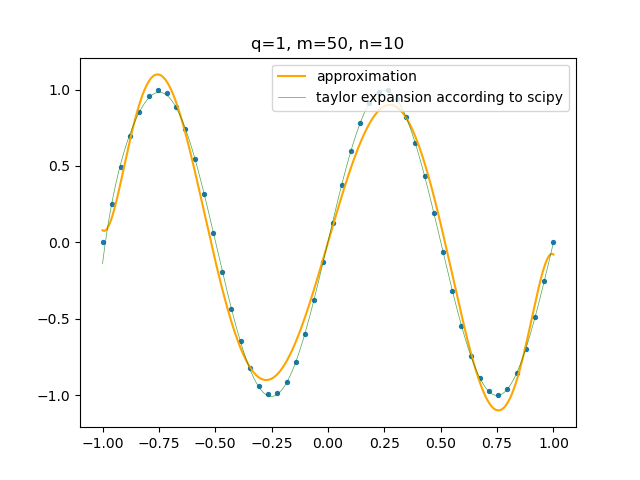
\includegraphics[width=72mm]{task_11} &   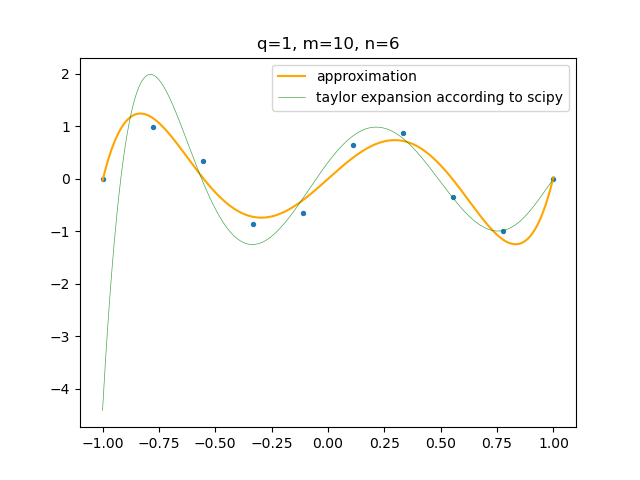
\includegraphics[width=72mm]{task_12} \\
                (a) task 11 & (b) task 12 \\[6pt]
            \end{tabular}
        \end{figure}

        \begin{figure}  
            \begin{tabular}{cc}
                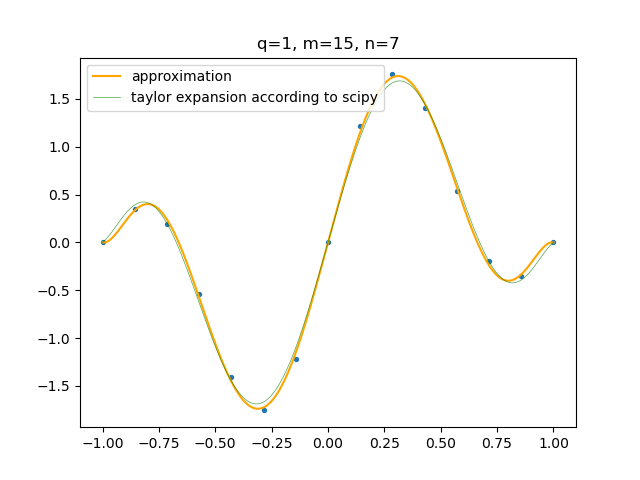
\includegraphics[width=72mm]{task_13} &   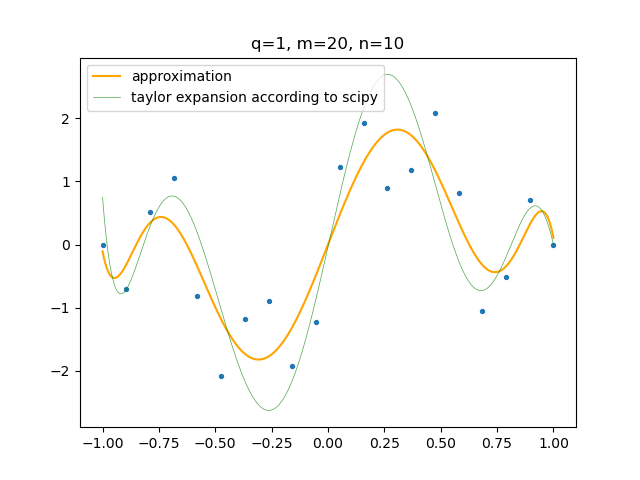
\includegraphics[width=72mm]{task_14} \\
                (a) task 13 & (b) task 14 \\[6pt]
            \end{tabular}
        \end{figure}
            
        \begin{figure}
            \begin{tabular}{cc}
                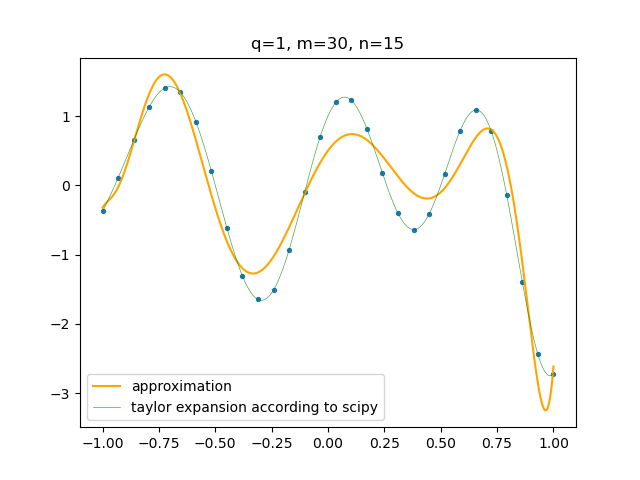
\includegraphics[width=72mm]{task_15} &   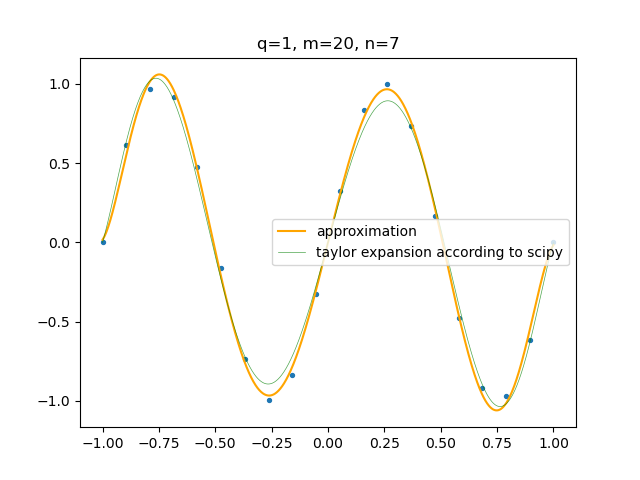
\includegraphics[width=72mm]{task_16} \\
                (a) task 15 & (b) task 16 \\[6pt]
            \end{tabular}
        \end{figure}

        \begin{figure}
            \begin{tabular}{cc}
                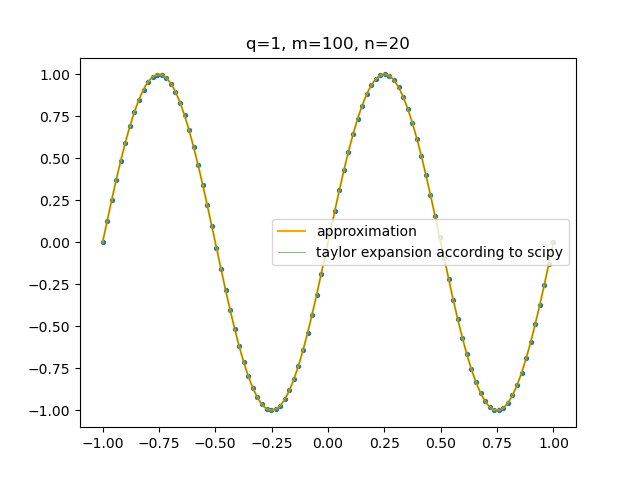
\includegraphics[width=72mm]{task_17} &   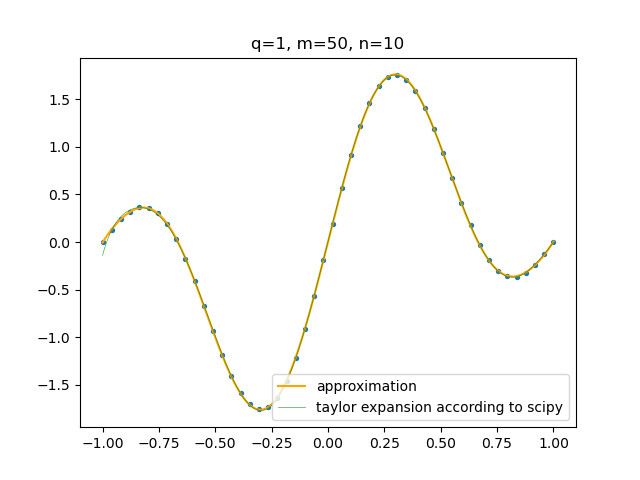
\includegraphics[width=72mm]{task_18} \\
                (a) task 17 & (b) task 18 \\[6pt]
            \end{tabular}
        \end{figure}
            
        \begin{figure}
            \begin{tabular}{cc}
                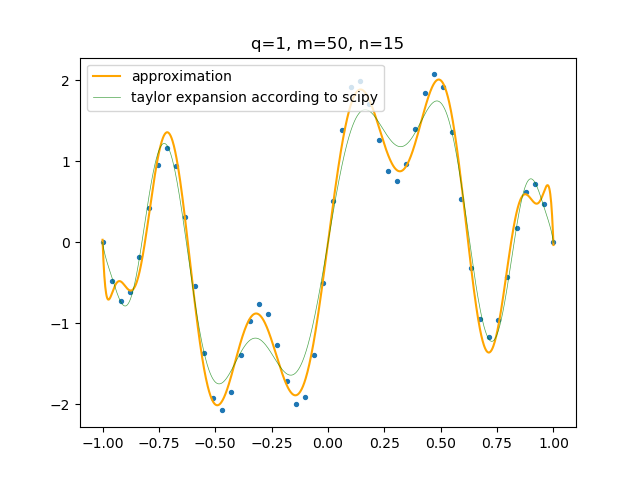
\includegraphics[width=72mm]{task_19} &   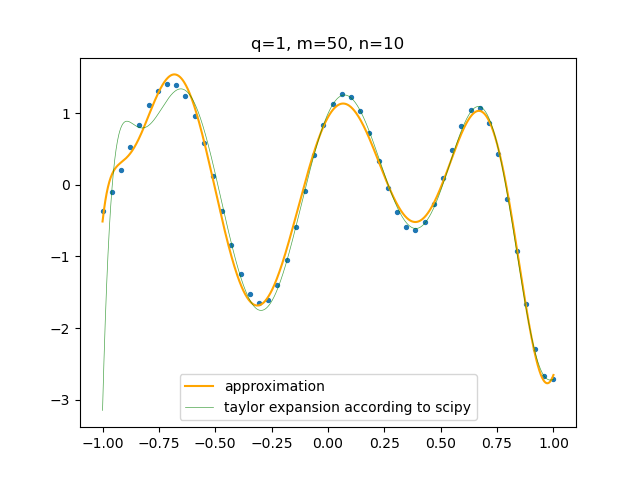
\includegraphics[width=72mm]{task_20} \\
                (a) task 19 & (b) task 20 \\[6pt]
            \end{tabular}
            \caption{Problem (ii)}
        \end{figure}

        % ------------------------------------------------------------------------
        \problem %(iii)
        I changed the stopping criterion from $\Vert \nabla f_k \Vert < 10^{-6}$ to $\Vert \nabla f_k \Vert < 10^{-2}$, otherwise convergence would take too long (maybe even infinite due to numerical imprecision). You can see this with the condition numbers. Due to this the results are not very good. The eigenvalues are obtained using \emph{numpy.linalg.eig}.

        \begin{table}[!ht]
            \tiny
            \begin{adjustbox}{angle=90}
                \begin{tabular}{|| c | c | p{3cm} | p{3cm} | c | c | p{3cm} | c | c | c ||} 
                    \hline
                    task & problem & $\{ x \in \mathbb{R}^n : x \text{ loc. min.}\}$ & $\tilde{x}$ & $\Vert f(\tilde{x}) \Vert$ & $\Vert \tilde{x} - x^* \Vert$ & eig.val. $\lambda_1, \dots, \lambda_n$ of $Q$ & $\frac{\lambda_n - \lambda_1}{\lambda_n + \lambda_1}$ & $\frac{\lambda_n}{\lambda_1}$ & iter. \\ [0.5ex] 
                    \hline\hline
                    21 & $n=5$ & \{ (5, -120, 630, -1120, 630) \} & (-2.3142, 31.4853, -62.0001,-35.2023, 85.1932) & 115.48 & 1405.51 & \{ 1.5670, 0.2085, 0.0114, 3.0589e-4, 3.2879e-06 \} & -0.9999 & 2.0981e-06 & 2038 \\
                    \hline
                    22 & $n=8$ & \{ (6, -278, 2717, -9684, 12439, 1804, -15160, 8207) \} & (0.8584, -25.0388, 91.8059, -12.0188, -101.0061, -98.9850, -1.1862, 175.4548) & 244.9215 & 23572.6820 & \{ 1.6959, 0.2981, 0.0262, 0.0014, 5.4369e-05, 1.2943e-06, 1.7988e-08, 1.1115e-10 \} & -0.9999 & 6.55412e-11 & 6885 \\
                    \hline
                    23 & $n=12$ & \{ (-7, 331, -3375, 12062, -13459, -6647, 9962, 13193, 950, -14225, -14724, 16022) \} & (2.7494, -28.2722, 23.9808, 65.6464, 30.9794, -32.4878, -84.1341, -103.1135, -82.2686, -21.9255, 74.0605, 200.5100) & 279.9208 & 36484.6892 & \{ 1.7953, 0.3802, 0.0447, 0.0037, 0.0002, 1.1163e-05, 4.0823e-07, 1.1228e-08, 2.2519e-10, 3.1113e-12, 2.6488e-14, 1.0955e-16 \} & -1.0 & 6.1023e-17 & 6880 \\
                    \hline
                    24 & $n=20$ & \{ (7, -349, 3436, -11386, 10140, 8391, -3849, -10825, -8635, -1102, 6793, 11234, 10599, 5554, -2205, -9789, -14105, -12393, -1784, 20405) \} & (2.5408, 37.9365, -83.6696, -40.7594, 41.9088, 92.5506, 97.5810, 67.2641, 17.4699, -37.4019, -86.4135, -122.1064, -139.8910, -137.3396, -113.5645, -68.7285, -3.6786, 80.3189, 181.7650, 299.0559) & 493.5051 & 41324.4256 & \{ 1.9071, 0.4870, 0.0755, 0.0089, 0.0008, 7.0334e-05, 4.8305e-06, 2.8276e-07, 1.4139e-08, 6.0360e-10, 2.1928e-11, 6.7408e-13, 1.7382e-14, 3.7547e-16, 1.3662e-17, 9.7897e-18, 1.1364e-18, -3.3954e-18+1.9338e-18j, -3.3954e-18-1.9338e-18j), -9.6106e-18 \} & -1.0 & -5.0392e-18 & 11725 \\
                    \hline
                    25 & $n=30$ & \{ (8, -272, 1979, -4326, 721, 3496, 2360, -279, -2436, -3272, -2835, -1537, 112, 1668, 2821, 3406, 3385, 2794, 1758, 431, -1010, -2376, -3491, -4184, -4299, -3694, -2260, 101, 3480, 7932) \} & (0.9888, -27.0951, 109.843 , -37.9596, -115.0667, -95.9121, -27.9969, 46.8452, 104.7627, 136.2247, 140.5346 121.6452, 85.4868, 38.4203, -13.5812, -65.3118, -112.46, -151.6005, -180.1179, -196.1031, -198.2434, -185.7175, -158.1018, -115.2882, -57.4151, 15.1907, 102.0612, 202.6263, 316.2444, 442.2279) & 828.3468 & 15980.9316 & \{ 1.9864, 0.5725, 0.1056, 0.0154, 0.0019, 0.0002, 1.9965e-05, 1.6986e-06, 1.2925e-07, 8.8280e-09, 5.4235e-10, 3.0008e-11, 1.4958e-12, 6.7143e-14, 2.7112e-15, 9.8549e-17, 1.2370e-17, 9.4688e-18, 8.0259e-18, 3.2087e-18, 2.8685e-18+1.0937e-18j, 2.8685e-18-1.0937e-18j, 9.7422e-19, -3.1024e-18, -4.3801e-18+3.4639e-18j, -4.3801e-18-3.4639e-18j, -5.9583e-18+1.4215e-18j, -5.9583e-18-1.4215e-18j, -7.5597e-18, -1.2380e-17 \} & -0.9999 & -6.2322e-18 & 25612 \\ [1ex] 
                    \hline
                \end{tabular}
            \end{adjustbox}
        \end{table}

        % ------------------------------------------------------------------------
        \problem %(iv)
        Tasks 26-30. The stopping criterion considers $\Vert \nabla f_k \Vert$.

        \begin{table}[!ht]
            \begin{adjustbox}{angle=90}
                \begin{tabular}{|| c | c | c | p{2cm} | c | c | c | c ||} 
                    \hline
                    task & problem & \footnotesize $\{ (x, y) \in \mathbb{R}^2 : (x, y) \text{ loc. min.}\}$ & $\tilde{x}$ & $\Vert f(\tilde{x}) \Vert$ & $\Vert \tilde{x} - x^* \Vert$ & \tiny stop crit. & iter. \\ [0.5ex] 
                    \hline\hline
                    26 & \footnotesize $(10 x_1 - 10x_2^2)^2 + (1 - x_0)^2$ & \{ (1,1) \} & \footnotesize (1., 1.) & 0.0 & 7.5e-01 & 1e-06 & 2 \\
                    \hline
                    27 & \footnotesize $(2x_1^2 - 8x_2)^2 + (x_1 - 1)^2$ & \{ (1, 1/4) \} & \footnotesize (1., 0.25) & 0.0 & 0.e+00 & 1e-06 & 2 \\
                    \hline
                    28 & $(10x_1^2 - 2.5x_2)^2 + (x_1 + 1)^2$ & \{ (-1, 2) \} & \footnotesize (-1., 2.) & 0.0 & 0.e+00 & 1e-18 & 2 \\
                    \hline
                    29 & $(10x_1 - 0.01x_2^2)^2 + (x_2 - 100)^2$ & \{ (10, 100) \} & \footnotesize (10., 100.) & 4.3e-30 & 0.e+00 & 1e-18 & 2 \\
                    \hline
                    30 & $(x_2 - x_1^2)^2 + (100 - x_1)^2$ & \{ (100, 10.000) \} & \scriptsize (100., 10000.00000001) & \scriptsize 3.5343e-21 & \scriptsize 1.1889e-08 & 1e-18 & 5 \\ [1ex] 
                    \hline
                \end{tabular}
            \end{adjustbox}
        \end{table}

    \end{enumerate}
\end{document}